\chapter{Definitions}
\label{chapter:definitions}

This chapter presents the definitions and notations used throughout this work. The definitions shown are based on \cite{BondyNMurty} and \cite{Diestel}.

\section{Graph Notations and Concepts}

A graph is a pair \(G = (V, E)\) of sets satisfying \(E \subseteq [V]^2\); that is, the elements of \(E\) are subsets of \(V\) with two elements. The elements of \(V\) are called vertices and of \(E\) are called edges.

The set of vertices of a graph $G$ are also denoted as \(V(G)\) and the set of edges as \(E(G)\). We express membership of a vertex \(v\) to a graph \(G\) with the notation \(v \in V(G)\), and similarly, for an edge \(e\), we denote \(e \in E(G)\). Alternatively, we can use \(v \in G\) or \(e \in G\) when the context makes it clear that we are referring to vertices or edges, respectively.

A vertex \(v\) is \textbf{incident} to an edge \(e\) if \(v \in e\); so \(e\) is an edge connected to \(v\). The two vertices incidents to \(e\) are called the \textbf{endpoints} of \(e\). Another notation commonly used to represent an edge \(\{v, w\}\) is by \(vw\) simply, where \(v, w \in V(G)\) are the endpoints.

The number of vertices of a graph is referred to as the graph's \textbf{order}, denoted by~\(|G|\). The number of edges is referred to as its \textbf{size} and is denoted by \(||G||\).

Two vertices \(u\), \(v\) of \(G\) are \textbf{adjacent} or \textbf{neighbors} if there is \(e \in E(G)\) such that \(u\) and \(v\) are its endpoints. Equivalently, two edges \(e\) and \(f\) are adjacent if they have one of their endpoints in common.

Let \(v \in V(G)\) be a vertex. We denote as \(N(v)\) the \textbf{open neighborhood} of \(v\), that is, the set of all vertices \(w \in V(G)\) such that \(w\) is adjacent to \(v\). The \textbf{closed neighborhood} of \(v\), denoted as \(N[v]\) is \(N(v) \cup \{v\}\).

If there is an edge \(uv \in E(G)\) for any pair of vertices \(u, v \in V(G)\),  then we say that \(G\) is a \textbf{complete} graph. A complete graph of \(n\) vertices is denoted as \(K^n\).

The \textbf{degree} of a vertex \(v\) is the number of edges of \(G\) incident to \(v\), denoted by \(d(v)\). If \(v\) is a vertex such that \(d(v) = 0\), we say that \(v\) is an \textbf{isolated vertex}. The number \(\delta(G) := \min \{d(v) \colon v \in V(G)\}\) is the \textbf{minimum degree} of \(G\); the number \(\Delta(G) := \max \{d(v) \colon v \in V(G)\}\) is the \textbf{maximum degree} of \(G\).

We say that a graph \(H\) is a \textbf{subgraph} of \(G\) if \(V(H) \subseteq V(G)\) and \(E(H) \subseteq E(G)\), and denote this by \(H \subseteq G\). If for any pair of vertices \(v, w \in H \subset G\), the statement \(vw \in E(H)\) is valid if, and only if, \(vw \in E(G)\), then we say that \(H\) is an \textbf{induced subgraph} of \(G\), denoted as \(G[H]\). Moreover, we say that \(H\) is a \textbf{spanning subgraph} of \(G\) if \(V(H) = V(G)\).

A \textbf{path} in a graph \(G\) is a sequence of distinct vertices \(P = (v_1, v_2, \dots, v_k)\), \(P \subseteq V(G)\), such that, for every pair of consecutive vertices of \(P\), there is an edge in \(E(G)\) that connects these vertices. That is, for every \(v_i , v_{i+1}\) in \(P\), there is \(v_i v _{i+1} \in E(G)\). The number of vertices in the path is its \textbf{length}, and a path of length \(k\) is denoted by \(P^k\).

Let \(C = (v_1, v_2 \dots, v_k)\) be a sequence of adjacent vertices such that \(|C| \geq 3\) and the endpoints of the sequence \(C\) are equal, that is, \(v_1 = v_k\), then we say that \(C\) is a \textbf{cycle}. The \textbf{length} of a cycle equals the number of edges in it. 

A \textbf{walk} (of length \textit{k}) is a non-empty alternating sequence \((v_0, e_0, v_1, e_1, \dots, e_{k-1}, v_k)\) of vertices and edges such that \(e_i = \{v_i, v_{i+1}\}\) for all \(i < k\). In particular, in the case \(v_0 = v_k\), we call it a \textbf{closed walk}. Note that, in a walk, vertices and edges can be visited more than once.

% In this work, the term ``cycle'' is used to denote a closed walk in a graph or, equivalently, the multiset of edges that form the walk. A noteworthy observation is that all vertices along the walk have even degrees, taking into consideration the repetitions of edges. Conversely, we call ``simple'' a cycle without edges repetition.

Given \(u, v \in V(G)\), if there is a path between \(u\) and \(v\) in \(G\), we say that the vertices are \textbf{connected}.

If there is a partition of \(V(G)\) into subsets \(V_1 , V_2 , \dots, V_w\) such that two vertices \(u\) and \(v\) are connected if, and only if, \(u\) and \(v\) belong to the same subset \(V_i\), then we say that the subgraphs \(G[V_1], G[V_2], \dots, G[V_w]\) are the \textbf{components} of \(G\). If \(G\) contains a single component, we say that \(G\) is \textbf{connected}, otherwise \(G\) is \textbf{disconnected}.

Let \(e \in E(G)\). We define as \textbf{contracting} the operation on \(e\) which consists on replacing both endpoints of \(e\) with a new vertice \(v_e\) and connecting \(v_e\) to \(e\) endpoint's neighboors.

We denote the graph obtained from \(G\) by \textbf{contracting} the edge \(e \in E(G)\) at a new vertex \(v_e\), which becomes adjacent to all old neighbors of the endpoint vertices of \(e\), as \(G / e\).

Given a graph \(G\) and a subgraph \(H\) of \(G\), we \textbf{contract} \(H\) into a single vertex \(v\), generating a new graph \(G^\ast := G / H\). All vertices of \(G - H\) adjacent to at least two vertices from \(H\) are connected to \(v\) in \(G^\ast\) with multiple edges. We also define the process of \textbf{uncontracting} \(v\) as replacing it with the original subgraph \(H\) and reconstructing the previous connections with the neighboring vertices of \(H\) in \(G\).

A collection \(\mathcal{S}\) is said to be \textbf{laminar} if and only if for any two sets \(C_1, C_2 \in \mathcal{S}\) we have \(C_1 \subseteq C_2\), or \(C_2 \subseteq C_1\), or \(C_1 \cap C_2 = \emptyset\). Suppose \(\mathcal{C}\) is a partition of a ground set \(V\). Then, \(\mathcal{C}(v)\) denotes, for each \(v \in V\), the set \(C \in \mathcal{C}\) that contains \(v\).

We define \(\ell \colon E(G) \to \mathbb{R}_\ge\), for \(e \in E(G)\) as the \textbf{length} (or cost) of \(e\). Naturally, \(\ell(H)\), for \(H \subseteq G\), is the sum of the cost of the edges of the subgraph \(H\). Let \(C = \{(v_1, v_2, \dots, v_k)\}\) be a cycle of \(G\). We define \(\ell(C) = \sum_{i=1}^{k-1} \ell(v_i v_{i+1})\).

For vertices \(v, w \in V(G)\) we define the \textbf{distance} between vertices $v$ and $w$, denoted by \(dist_G(v, w)\), as the length of a shortest path between \(v\) and \(w\) that only uses edges of \(G\). If such a path does not exist, by convention, we consider \(dist_G(v, w) = +\infty\). We generalize the notation for distances between vertices and edges. Let \(v \in V(G)\) and \(uw \in E(G)\). Define the distance between the vertex \(v\) and the edge \(uw\) as \(dist_G(v, uw) := \min\{dist_G(v, u), dist_G(v, w)\} + \ell(uw)\).

% This notation follows naturally for a subgraph \(G'\) of \(G\), where given \(v, u \in V(G')\), \(dist_{G'}(v, u)\) is the length of a shortest path that only transverse edges in \(G'\) between the vertices \(v\) and \(u\).

A graph \(F\) without cycles is a \textbf{forest}. A connected forest is a \textbf{tree}. Let \(T\) be a tree and \(v \in T\) a vertex. If \(d(v) = 1\), we say that \(v\) is a \textbf{leaf} of \(T\), all other vertices are called inner vertices of \(T\). A tree is rooted if one of its vertices has been chosen as \textbf{root}. Naturally, a forest's component is a tree. 

Let \(T\) be a rooted tree with root \(r \in V(T)\), let \(v \in V(T)\). Note that there is only a single path between \(r\) and \(v\) in \(T\). Let \(P\) be this unique path between \(v\) and \(r\). We say that \(w \in V(T)\) is the \textbf{parent vertex} of \(v\) if \(w \in P\) and \(w \in N(v)\). Equivalently, we say that \(v\) is a \textbf{child vertex} of \(w\). Note that a vertex can have multiple children but only one parent.

Given a connected graph \(G\), we say that a \textbf{shortest-path tree} \(SPT\) rooted at a vertex \(v\) of \(V(G)\) is a spanning tree of \(G\) such that the path distance from root \(v\) to any other vertex \(u \in V(SPT)\) is a shortest path from \(v\) to \(u\) in \(G\), i.e., \(dist_{SPT}(u, v) = dist_{G}(u, v)\).

As defined by~\cite{ROBERTSON1986309}, a \textbf{tree decomposition} of \(G\) is a pair \((T, B)\) in which \(T\) is a tree and \(B = \{B_i \colon i \in V(T)\}\) is a family of subsets of \(V(G)\), so that:

\begin{itemize}
    \item \(\bigcup_{i \in V(T)} B_i = V(G)\);
    \item For each edge \(uv \in E(G)\), there is a \(i \in V(T)\) such that \(u, v \in B_i\);
    \item For each \(v \in V(G)\), the set of vertices \(\{i \in V(T) \colon v \in B_i\}\) forms a subtree of \(T\).
\end{itemize}

To differentiate from the original graph \(G\), we call the vertices of \(T\) \textbf{nodes}, where each node \(i\) has a corresponding \textbf{bag} of vertices \(B_i\). An example can be seen in Figure~\ref{fig:decomp1}.

\begin{figure}[H]
    \centering
    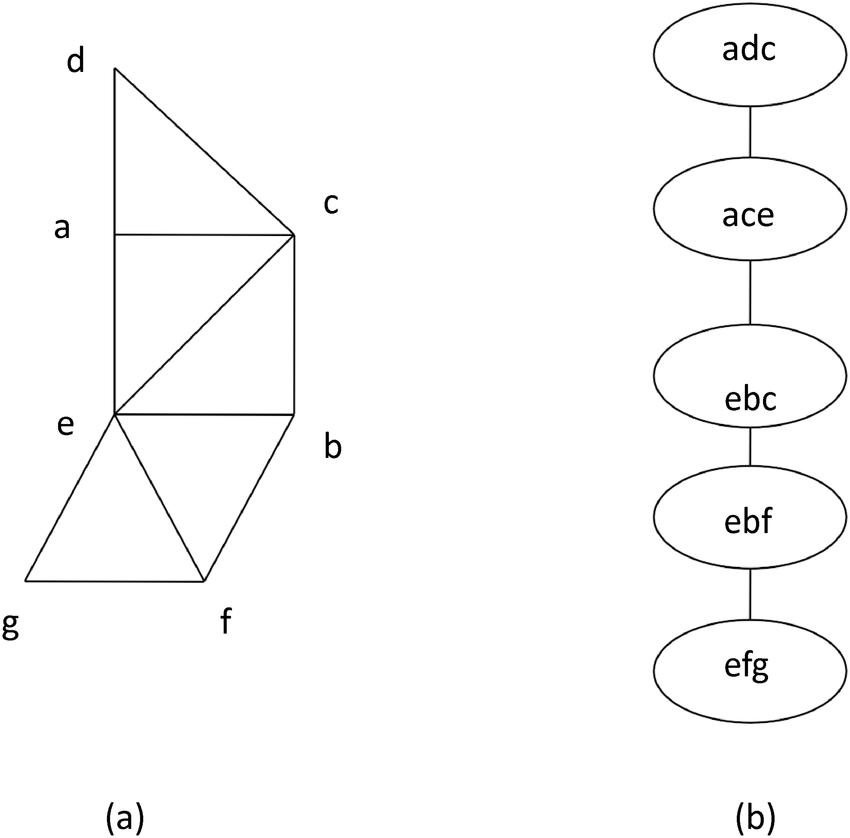
\includegraphics[scale=2]{imgs/decomp1.png}
    \caption{Example of a graph and its tree decomposition.~(\cite{imgTreeDecomp}).}
    \label{fig:decomp1}
\end{figure}

The \textbf{width} of a tree decomposition is the size of its largest bag minus one. The \textbf{treewidth} of a graph \(G\), denoted with \(tw(G)\), is the smallest width of a tree decomposition of \(G\).

To facilitate application in algorithms, we focus on a more restricted class of decompositions. We say that a tree decomposition \((T, B)\) is \textbf{nice} when \(T\) is a rooted tree and each \(i \in V(T)\) belongs to one of the following classes:

\begin{itemize}
    \item \(i\) is a \textit{leaf node} if it has no children;
    \item \(i\) is a \textit{union node} if \(i\) has exactly two children \(i_1, i_2\) and it holds \(B_i = B_1 = B_2\);
    \item \(i\) is an \textit{introduction node} if it has a single child \(i'\) and it holds \(B_i = B_{i'} \cup \{v\}\) for some vertex \(v \in V(G)\);
    \item \(i\) is a \textit{forgetting node} if it has a single child \(i'\) and it holds \(B_i = B_{i'} \backslash \{v\}\) for some vertex \(v \in V(G)\).
\end{itemize}

Given two bags \(B_i\) and \(B_j\), we say that \(B_j\) is a \textbf{descendant} of \(B_i\) if it is separated from the root bag by \(B_i\).

\section{Graph Planarity and Genus}

Informally, we characterize as \textbf{planar} a graph \(G\) that can be drawn on a plane without its edges intersecting outside their endpoints. Thus, the graph can be seen as points on a surface (vertices) with arcs (edges) connecting the points in such a way that arcs do not intersect outside a point. The surface region surrounded by arcs is called a \textbf{face} of the graph. Moreover, the outer region of the graph is the \textbf{outer face}, while all other faces are \textbf{inner faces} of \(G\). The \textbf{boundary} of \(G\) is the set of edges that separate the outer face of \(G\) from the rest of the graph, is denoted by \(\partial(G)\).

Formally,~\cite{Diestel} defines a planar graph as a pair \((V, E)\) of finite sets with the following properties:

\begin{itemize}
    \item \(V \subseteq \mathbb{R}^2\);
    \item every edge is an arc between two vertices;
    \item different edges have a different set of extreme points;
    \item The interior of an edge does not contain vertices or intersections with other edges.
\end{itemize}

For any planar graph, the set \(\mathbb{R}^2 \backslash G\) is open, and its regions are the faces of \(G\).

The intuitive idea of ``drawing'' a planar graph into a ``plane'' is what we call a \textbf{planar embedding} of \(G\). According to~\cite{Diestel}, an embedding in the plane of an (abstract) graph \(G\) is an isomorphism between \(G\) and a \textbf{plane graph} \(\tilde{G}\). The latter is referred to as \textbf{drawing} of \(G\).

\cite{BondyNMurty} showed that a planar embedding of a graph \(G\) exists if and only if \(G\) is also embeddable on the sphere. This idea will be useful to generalize the concept of embedding graphs to other surfaces.

Formally, they define a \textbf{surface} as a 2-dimensional manifold. We will skip a more detailed presentation of the topological definitions and properties of this structure, as for the reader it suffices to know that a sphere is a surface, as well as a torus and other constructions formed by pushing additional ``holes'' in the sphere. The number of ``holes'' in the sphere is what we call the \textit{genus} of the surface.

// TODO mencionar resultado que eh possivel determinar se um grafo eh planar em tempo polinomial

Informally, we say that the \textbf{genus} of a graph is the smallest number \textit{g} such that the graph can be drawn on a sphere with \textit{g} holes without edges crossing. From this idea, a planar graph has genus 0.

Interestingly, the problem of determining the genus of a graph is known to be \(\nonpoly\)-complete (\cite{THOMASSEN1989568}). However, as presented by \cite{LinearGenus}, the problem becomes treatable when the genus \textit{g} is fixed; that is, we can determine in polynomial time whether a graph can be embedded in a surface with genus \textit{g}, considering \textit{g} constant. As a secondary result, the authors also present a linear time algorithm, which computes the genus and constructs minimum genus embeddings of graphs of bounded treewidth. 

For a given planar graph \(G\), we say that \(H\) is its \textbf{dual} if there is a bijective function that maps the faces of \(G\) to the vertices of \(H\) and, for each edge \(e \in E(G)\) that separates the faces \(f\) and \(f'\) of \(G\), we have an edge that connects the vertices associated to \(f\) and \(f'\) in \(H\).

The concept of \textbf{faces} can be generalized to higher \textit{genus} graphs when we embed the graph on a surface of same genus.

\section{Classes of Optimization Problems}

In combinatorial optimization problems, we want to obtain the best solution from a finite, but potentially large, set of possible solutions. \cite{livroAprox} defined an optimization problem with the following elements: a set of instances, a set \(\sol(I)\) of viable solutions for a given instance \(I\), and a function \(\val (I, S)\) that associates to each instance and solution \(S \in \sol(I)\) a non-negative rational value. The solution to the optimization problem is the \(S\) that minimizes/maximizes \(\val(I, S)\).

More formally, for a given instance \(I\) there is a solution \(S^* \in \sol(I)\) such that \(\val(I, S^*) \leq \val(I, S)\) for all \(S \in \sol(I)\), considering a minimization scenario. The idea follows equivalently for a maximization problem. We denote \(\opt := \val(I, S^*)\) as the value of the optimal solution of \(I\). In particular, for the problems discussed in this work, we denote as \(\opt_{\mathcal{T}}(G)\) the value of an optimal solution in the graph \(G\) considering a set of pairs of terminals \(\mathcal{T}\).

There is an intimate relationship between the classes of optimization problems and the well-known classes of decision problems \(\poly\), \(\nonpoly\), \(\nonpoly\)-hard, \(\nonpoly\)-complete. There are optimization problems for which there are limitations of the approximability of their solutions by polynomial algorithms, considering \(\poly \neq \nonpoly\).

That said, optimization problems are classified according to their degree of approximability. By approximability, we observe a scenario in which we give up finding an optimal solution in favor of finding a solution that, while sub-optimal, can be found efficiently and maintain quality guarantees. We will consider and detail the classes PO, PTAS (and its variants QPTAS, FPTAS, and EPTAS), APX, and NPO, as described by \cite{livroAprox}.

According to \citeauthor{livroAprox}, the NPO class, which is an extension of the \(\nonpoly\) class for optimization problems, is composed of the problems where:

\begin{itemize}
    \item There is a polynomial function \textit{p} such that the size of the solution \(S\) is less or equal to the size of the instance \(I\) applied on \textit{p}, for every instance \(I\) of the problem and every feasible solution \(S\) of \(I\);
    \item There is a polynomial time algorithm that decides whether a given word is a valid representation of an instance of the problem;
    \item There is a polynomial time algorithm that decides whether a given object is a feasible solution for a given instance of the problem;
    \item There is a polynomial time algorithm that calculates \(\val(I, S)\), given \(I\) and \(S\).
\end{itemize}

We denote as PO the class of problems treatable in polynomial time. This class is an extension of the \(\poly\) class for optimization problems. Therefore, given a pro[blem \(\pi\), we say that \(\pi \in PO\) if there is a polynomial time algorithm that calculates an optimal solution for each instance \(I\) of \(\pi\). Examples of problems in this class are the Shortest Path and Minimum Spanning Tree problems.

Consider an optimization problem. Let \(A\) be an algorithm that for every instance \(I\) of the problem returns a feasible solution \(A(I)\) of \(I\). If the problem is one of minimization and \(val(I, A(I)) \leq \alpha \opt\) holds for every instance \(I\), then we say that \(A\) is a \textbf{\(\alpha\)-approximation} for the problem. We define \(\alpha\) as the \textbf{approximation ratio} of the algorithm.

The APX class comprises optimization problems in NPO for which there is an \(\alpha\)-approximation for some constant \(\alpha\). One of the most famous algorithms that provide this type of approximation is the Christofides Algorithm, developed by~\cite{Christofides2022WorstCaseAO} to the TSP problem restricted to metric graphs and which guarantees an approximation ratio of \(\alpha = 1.5\).

For a given optimization problem, we define as an \textbf{approximation scheme} an algorithm that receives an instance \(I\) of the problem as well as a parameter \(0 < \epsilon < 1\) and returns a solution \(S\) such that \(\val(I, S) \leq (1 + \epsilon) \opt\), for a minimization problem. We say that an algorithm is a \textbf{polynomial-time approximation scheme} (PTAS) if it has polynomial time for every fixed \(\epsilon\). Furthermore, an algorithm is a \textbf{fully polynomial-time approximation scheme}, or FPTAS, if its time is also polynomial in \(1 / \epsilon\). In contrast, a PTAS algorithm which is not FPTAS is exponential in \(1 / \epsilon\).

We will briefly comment on two other PTAS classes of interest. An \textbf{efficient polynomial-time approximation scheme} (EPTAS) is a more relaxed version of the FPTAS, where the complexity on \(1 / \epsilon\) does not need to be polynomial. I.e., a PTAS algorithm with time complexity \(\mathcal{O}(c^{1 / \epsilon} n^k)\), for \(c\) and \(k\) constants, is an EPTAS.

Another class worth mentioning is the \textbf{quasi-polynomial-time approximation scheme} (QPTAS), which allows a sub-linear factor as an exponent, i.e., an algorithm with time-complexity \(\mathcal{O}(c^{\log{n}})\) for every fixed \(\epsilon\) and where \(c\) is a constant.

From the definitions, it follows that \[PO \subseteq FPTAS \subseteq PTAS \subseteq APX \subseteq NPO.\]
